\renewcommand{\nomebreve}{hanoi\_equal\_disks}
\renewcommand{\titolo}{The Hanoi puzzle with equal disks}

\introduzione{}

Se non conosci il puzzle classico della torre di Hanoi, o la descrizione quì sotto non basta, chiedi spiegazione in aula.

\begin{figure}[h!]
\begin{center}
  \noindent 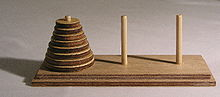
\includegraphics[width=0.57\textwidth]{figures/220px-Tower_of_Hanoi.jpeg}
\end{center}
\caption{Configurazione iniziale del puzzle classico della torre di Hanoi.}
\end{figure}

Ci sono tre pioli ('A','B' e 'C') su cui trovano collocazione $n$ dischi, numerati da $1$ ad $n$, come presi dal più piccolo al più grande. Le configurazioni valide sono quelle in cui nessun disco si trova collocato sopra un disco più piccolo.
Viene richiesto di portarsi dalla configurazione in cui tutti i dischi risiedono sul piolo 'A' (detta \it{configurazione iniziale}) alla \it{configurazione finale} in cui tutti i dischi sono in 'B', spostando sempre un solo disco alla volta (mossa) e visitando solo configurazioni valide.
\'E nota l'elegante soluzione ricorsiva che risolve il puzzle classico (Édouard Lucas, 1883) col minimo numero di mosse. La soluzione ottima è di fatto unica anche se trova diverse descrizioni/rappresentazioni/interpretazioni in forma iterativa.

\begin{center}
  \animategraphics[loop,autoplay]{12}{./figures/animation/frame-}{0}{39}
\end{center}

Quì ti chiediamo di analizzare il caso più generale quando possano aversi dischi delle stesse dimensioni.

Quindi ora il disco~$j$, con $j>i$, può anche essere disposto sopra il disco disco~$i$ qualora il diametro dei due dischi sia precisamente lo stesso.

In realtà vogliamo valutare almeno un paio di competenze. Nei subtask di tipo~$t=1$ ti chiediamo di listare tutte le mosse di una soluzione ottima, che porti tutti i dischi in 'B' impiegando il minor numero di mosse.
Nei subtask di tipo~$t=0$ ti chiediamo solamente di computare tale numero di mosse, senza doverle generare, ma più velocemente.
Nel primo caso consigliamo un approccio ricorsivo e nel secondo un approccio iterativo.
Consigliamo di affrontare prima i subtask di tipo~$t=1$.


\sezionetesto{Input ed Output}

Per la gestione pulita di input ed output consigliamo di utilizzare il template di soluzione fornito tra gli attachmets alla pagina del problema.
Input ed output avvengono da \verb'stdin'
e da \verb'stdout' rispettivamente.
La prima riga dell'input contiene i due numeri $t$ ed $n$, nell'ordine e separati da spazio. Questi indicano il tipo di richiesta (solo contare o proprio listare le mosse) ed in numero di dischi.
Nella seconda riga sono riportati $n$ numeri interi positivi, i diamentri degli $n$ dischi riportati nell'ordine (dal disco~$1$ al disco~$n$) e separati da spazio. Pertanto tale sequenza risulta essere monotona non-decrescente.
Nel caso in cui $t=0$, il vostro programma deve restituire su \verb'stdout' un unico numero naturale: il minimo numero di mosse che è necessario spendere per portare tutti i dischi sul piolo 'B'.
(Ricodiamo che la configurazione iniziale vede gli $n$ dischi tutti impilati sul piolo 'A', ordinati per etichetta.
Altrimenti, nel caso in cui $t= 1$,
allora il vostro programma deve riportare su \verb'stdout'
la più breve sequenza di mosse che consente di portare tutti i dischi sul piolo 'B', come più precisamente illustrato negli esempi. 


% Esempi
\sezionetesto{Esempio di input/output}

In attachment alla pagina del problema trovate diverse copie input/output tra cui le seguenti.


\vspace{0.5cm}
\esempio{
0 4

1 2 2 5

}{9}

\vspace{0.5cm}
\esempio{
1 4

1 2 2 5

}{sposta il disco 1 dal piolo A al piolo B

sposta il disco 2 dal piolo A al piolo C

sposta il disco 3 dal piolo A al piolo C

sposta il disco 1 dal piolo B al piolo C

sposta il disco 4 dal piolo A al piolo B

sposta il disco 1 dal piolo C al piolo A

sposta il disco 2 dal piolo C al piolo B

sposta il disco 3 dal piolo C al piolo B

sposta il disco 1 dal piolo A al piolo B
}

% Assunzioni
\sezionetesto{Assunzioni e note}
\begin{itemize}[nolistsep, noitemsep]
  \item $1 \le n \le 100\,000$.
\end{itemize}
  
\section*{Subtask}

  \begin{itemize}
    \item \textbf{Subtask 1 [0 punti]:} i casi di esempio forniti alla pagina del problema, essi includono i due casi sopra.
    \item \textbf{Subtask 2 [10 punti]:} $t=1$, $n \le 10$, diametri dei dischi tutti diversi.
    \item \textbf{Subtask 3 [10 punti]:} $t=1$, $n \le 15$, diametri dei dischi tutti diversi.
    \item \textbf{Subtask 4 [20 punti]:} $t=1$, $n \le 10\,000$, le mosse necessarie sono al più $100\,000$.
    \item \textbf{Subtask 5 [10 punti]:} $t=0$, $n \le 10$, diametri dei dischi tutti diversi.
    \item \textbf{Subtask 6 [10 punti]:} $t=0$, $n \le 16$, diametri dei dischi tutti diversi.
    \item \textbf{Subtask 7 [20 punti]:} $t=0$, $n \le 100\,000$, le mosse necessarie sono al più $1\,000\,000$.
    \item \textbf{Subtask 8 [20 punti]:} $t=0$, $n \le 100\,000$, le mosse necessarie sono al più $10\,000\,000\,000$.
  \end{itemize}
  
